\documentclass[11pt,a4paper]{article}
\usepackage{amsmath}
\usepackage{fontspec}
\setmainfont{Charter}
\setsansfont{Helvetica Neue}
\usepackage[margin=2.3cm]{geometry}
\usepackage{xcolor}
\usepackage{booktabs}
\usepackage{tabularx}
\usepackage{array}
\usepackage{enumitem}
\usepackage{microtype}
\usepackage{titlesec}
\usepackage{caption}
\usepackage{fancyhdr}
\usepackage{tikz}
\usepackage{parskip}
\usepackage[hidelinks]{hyperref}

\definecolor{ink}{HTML}{1F2933}
\definecolor{muted}{HTML}{616E7C}
\definecolor{accent}{HTML}{0B6E4F}
\definecolor{warn}{HTML}{B7791F}
\definecolor{risk}{HTML}{B83227}
\definecolor{panel}{HTML}{F2F5F3}
\color{ink}

\titleformat{\section}{\sffamily\Large\bfseries\color{accent}}{\thesection}{0.6em}{}
\titleformat{\subsection}{\sffamily\large\bfseries}{\thesubsection}{0.6em}{}
\titlespacing*{\section}{0pt}{1.4em}{0.5em}
\titlespacing*{\subsection}{0pt}{1.0em}{0.3em}
\captionsetup{font={small,sf},labelfont=bf}
\setlist{itemsep=0.2em,topsep=0.3em}

\pagestyle{fancy}
\fancyhf{}
\renewcommand{\headrulewidth}{0pt}
\fancyfoot[L]{\sffamily\footnotesize\color{muted}Economic Viability Index -- ETHack 2026}
\fancyfoot[R]{\sffamily\footnotesize\color{muted}\thepage}

\newcommand{\keybox}[2]{%
  \par\noindent\colorbox{panel}{\parbox{\dimexpr\linewidth-2\fboxsep}{%
  \vspace{0.35em}\sffamily\bfseries #1\par\vspace{0.2em}\normalfont\rmfamily #2\vspace{0.35em}}}\par}
\newcommand{\code}[1]{\texttt{\small #1}}
\newcolumntype{L}{>{\raggedright\arraybackslash}X}

\begin{document}

\begin{titlepage}
\vspace*{3cm}
{\sffamily\color{accent}\bfseries\large ETHack 2026 -- S\&P 500 sustainability}\par\vspace{0.6em}
{\sffamily\bfseries\fontsize{30}{36}\selectfont Economic Viability Index\par}
\vspace{0.8em}
{\Large How we got to the score -- and why it does not reward profit\par}
\vspace{2.5cm}
\keybox{In one sentence}{The index asks whether a company can keep paying its workforce, suppliers and lenders out of its own operations, including through a repeat of the worst year it has already been through. It uses only reported figures, stops giving credit once a company has ``enough'', and lets the weakest dimension set the verdict.}
\vfill
{\sffamily\color{muted} 12 September 2026\\
Data: SEC EDGAR XBRL companyfacts, 503 index constituents, fiscal years 2016--2026\\
Code: \code{fetch\_sec\_facts.py}, \code{financial\_health.py}, \code{economic\_viability.py} (branch \code{feat/economy})}
\end{titlepage}

\tableofcontents
\vspace{1em}
\keybox{Result at a glance}{%
\begin{tabular}{@{}lr@{\hspace{2.5em}}lr@{}}
Viable & 378 & Not assessable (banks, insurers, new registrants) & 77\\
Strained & 29 & Correlation with company size (Spearman $\rho$) & 0.03\\
At risk & 19 & Correlation with profit margin (Spearman $\rho$) & 0.12\\
\end{tabular}}

\clearpage
\section{The question}

A sustainability ranking of the S\&P 500 already measures environmental and social outcomes. What it did not measure is whether a company is economically able to \emph{continue}: to keep people employed and paid, to pay its suppliers, to service its debt. A company that ranks well on emissions but cannot fund its own operations is not sustainable in any practical sense.

The obvious yardstick -- profit -- answers a different question. A company that earns more than any other is not thereby more sustainable; beyond the point where it can reliably pay its obligations, additional profit says nothing about whether the workforce is safe. The index is therefore built around \textbf{capacity}, not magnitude:

\begin{enumerate}
  \item \textbf{Capacity, not size or profit.} Every measure is a ratio against the company's own obligations or its own history, and every score saturates at a level that counts as sufficient. There is no margin, return or growth metric.
  \item \textbf{Observed, not forecast.} Only figures from mandatory SEC filings. No analyst estimates, no market prices, no projections. The stress case is not an assumption but a repeat of the worst year the company has itself been through.
  \item \textbf{Weakest link.} A large cash pile does not buy back a decade of negative cash flow. Dimensions are combined geometrically and the verdict follows the weakest one.
\end{enumerate}

\section{How we got here: four iterations}

The final design is the fourth iteration. Each earlier version was tested against the data and rejected or reworked for a measurable reason. They are documented because the reasons explain the design.

\subsection{Attempt 1: a profit-weighted health score}
The first screen combined net margin, free cash flow margin, return on assets, debt payback years, revenue growth and interest coverage into a 0--100 score (\code{financial\_health.py}). It was useful as a financial overview, but it rewards exactly what should not be rewarded: a company with a 60\,\% margin scores far above one with a 10\,\% margin even when both can comfortably pay their staff. It also misreads loss-making companies with strong cash positions -- Intel, with a net loss of \$11.3\,bn over the last twelve months, scored 25.8 out of 100, although it held \$29.7\,bn in cash and generated \$14.9\,bn of operating cash flow.

\subsection{Attempt 2: ``six months of costs in cash''}
The first viability draft measured how many months of cash operating costs a company holds in cash if revenue stopped entirely, with six months counting as sufficient. The data rejected it:
\begin{itemize}
  \item the median S\&P 500 company holds \textbf{1.5 months}; healthy firms rely on credit lines and continuous cash flow rather than cash piles;
  \item 246 of 492 companies landed in ``at risk'', 172 of them solely because of this metric -- including Thermo Fisher and Cognizant, both cash-positive in ten out of ten years;
  \item a revenue stop of 100\,\% is not an observed event, it is a speculative scenario.
\end{itemize}
The measure survives only as an information column (\code{info\_cash\_months\_of\_costs}).

\subsection{Attempt 3: revenue stability}
A dimension based on the worst year-over-year revenue drop mostly measured things that do not threaten payroll: spin-offs and divestitures (DuPont $-74\,\%$, GE $-48\,\%$), commodity price cycles in oil and gas, and breaks in how companies tag revenue in XBRL (Camden Property Trust $-99\,\%$). It was dropped. The cash-flow history already contains the swings that actually mattered.

\subsection{Attempt 4: stress against the company's own worst year}
A stress test built on revenue (``lose your worst revenue drop, keep all costs'') penalised pass-through businesses such as McKesson or Cardinal Health, whose purchasing costs fall with sales. The fix was to stress operating \emph{cash flow} instead, because the historical fall in cash flow already reflects how a company's costs really adjusted. Scaling the historical fall by revenue or by total assets gave the same share of companies surviving a repeat (86\,\% in both cases); assets were chosen because revenue scaling breaks on revenue collapses (Moderna's worst year would have been 367\,\% of revenue) and on revenue-tag changes.

\section{Data}

\subsection{Source}
All figures come from the SEC's XBRL \emph{companyfacts} API, one file per company, downloaded for all 500 unique CIKs of the 503 constituents (plus ExxonMobil's pre-2026 predecessor registrant). It contains every tagged value from every 10-K, 10-Q, 8-K and proxy statement. We use:
\begin{itemize}
  \item \textbf{fiscal years}: periods of 350--380 days, from any filing except 10-Qs (some 10-Qs report trailing twelve months, which must not be mistaken for a fiscal year), the last ten per company;
  \item \textbf{trailing twelve months (TTM)}: last fiscal year $+$ current year-to-date $-$ prior year-to-date; 420 companies have periods ending June 2026 or later;
  \item \textbf{balance sheet}: the latest reported date, mostly 30 June 2026.
\end{itemize}

\subsection{Data problems found and fixed}
\begin{itemize}
  \item \textbf{Newest copy of a 10-K figure sits in a proxy statement or 8-K recast} (Nvidia, Cencora). Fix: accept any form for fiscal years; the period length decides.
  \item \textbf{Zero placeholders in predecessor/successor columns} (Paramount Skydance). Fix: a non-zero value beats a zero for the same period.
  \item \textbf{Company re-registered under a new CIK} (ExxonMobil). Fix: merge the predecessor's filings.
  \item \textbf{Debt tagged with company-specific elements} (Air Products, GM, Ford). Fix: fallback tags, each validated against reported long-term debt where both exist (share within $\pm$15\,\%): sum of the debt maturity schedule 94\,\%, long-term debt including current maturities 92\,\%, debt instrument carrying amount 88\,\%, debt and lease obligations 81\,\%.
  \item \textbf{A 10-Q reports a twelve-month figure} (Amazon). Fix: 10-Qs are excluded from fiscal-year detection.
\end{itemize}

\section{The three dimensions}

\subsection{Cash generation -- does the company fund itself?}
A company that does not bring in cash from operations lives on outside money: new debt, new shares or asset sales. Three components, averaged:
\begin{itemize}
  \item \textbf{track record}: share of the last ten fiscal years with positive operating cash flow;
  \item \textbf{asset upkeep}: share of years in which operating cash flow at least covered depreciation, i.e.\ the company could replace what wears out without outside money;
  \item \textbf{now}: operating cash flow positive over the trailing twelve months \emph{and} in each of the last three fiscal years (1.0), TTM positive but a recent negative year (0.5), TTM negative (0).
\end{itemize}
The ``now'' component was added after the first full run: without it, Netflix, Uber and Palantir were rated ``at risk'' for cash burn that ended years ago.

\subsection{Shock absorption -- could it get through its worst year again?}
This is the most direct translation of ``can it keep paying its workforce''. For every pair of consecutive fiscal years we compute the fall in operating cash flow as a share of total assets at the start of the year. The largest fall is the company's own observed worst case. We then ask what happens if it repeats today:
\[
\text{OCF}_{\text{shock}} = \text{OCF}_{\text{TTM}} - \text{worst fall share} \times \text{total assets today}
\]
If $\text{OCF}_{\text{shock}} \ge 0$, operating cash still covers the year and the score is 1. Otherwise the gap must come from cash, and
\[
\text{coverage} = \frac{\text{cash} + \text{short-term investments}}{-\text{OCF}_{\text{shock}}}
\]
measures how much of that gap existing cash covers without new borrowing, layoffs or asset sales.

\subsection{Debt service -- do lenders get paid without refinancing?}
Two components, averaged:
\begin{itemize}
  \item \textbf{interest burden}: cash interest paid as a share of operating cash flow before interest;
  \item \textbf{near-term maturities}: debt due within twelve months (current portion of long-term debt, short-term borrowings, commercial paper) divided by cash plus one year of operating cash flow.
\end{itemize}

\subsection{What is deliberately not scored}
\begin{itemize}
  \item \textbf{Profit, margin, growth, size.} They measure how much, not whether enough.
  \item \textbf{Revenue swings.} See section 2.3.
  \item \textbf{Payroll directly.} Only 71 companies tag labour expense in XBRL; it is kept as an information column. Payroll is part of the operating costs covered by operating cash flow.
  \item \textbf{Banks and insurers.} Deposits, trading assets and premiums make operating cash flow, liquidity and debt ratios mean something else. Scoring them would need regulatory capital data (FFIEC call reports, NAIC statements). They are marked \emph{not assessable} rather than scored with the wrong yardstick.
\end{itemize}

\section{From measures to a score}

\subsection{Saturating thresholds}
Each measure is converted to a score between 0 and 1 by a linear ramp between a ``zero'' point and a ``sufficient'' point. Beyond the sufficient point, nothing more is added. This is the mechanism that keeps profit from being rewarded: 42\,\% of assessed companies reach the maximum on every dimension, and they are all treated as equally viable.

\begin{figure}[h]
\centering
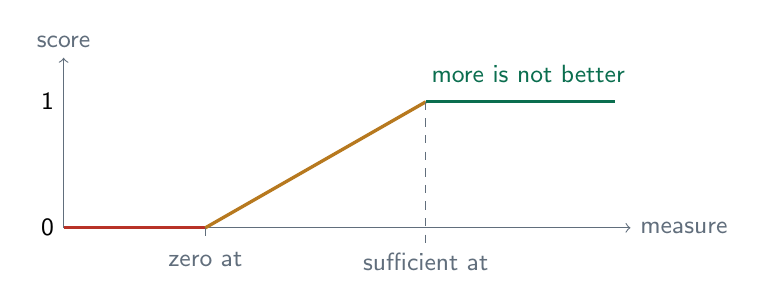
\begin{tikzpicture}[x=1cm,y=1.6cm,font=\sffamily\small]
  \draw[->,muted] (0,0) -- (7.2,0) node[right] {measure};
  \draw[->,muted] (0,0) -- (0,1.35) node[above] {score};
  \draw[very thick,risk] (0,0) -- (1.8,0);
  \draw[very thick,warn] (1.8,0) -- (4.6,1);
  \draw[very thick,accent] (4.6,1) -- (7,1);
  \draw[dashed,muted] (1.8,0) -- (1.8,-0.12) node[below] {zero at};
  \draw[dashed,muted] (4.6,1) -- (4.6,-0.12) node[below] {sufficient at};
  \node[left] at (0,1) {1};
  \node[left] at (0,0) {0};
  \node[accent,align=center] at (5.9,1.22) {more is not better};
\end{tikzpicture}
\caption{Every measure is scored on a ramp that stops at a ``sufficient'' level.}
\end{figure}

\begin{table}[h]
\centering\small
\begin{tabularx}{\linewidth}{@{}lLrr@{}}
\toprule
Dimension & Measure & Score 0 at & Score 1 at \\
\midrule
Cash generation & share of years with positive operating cash flow & 50\,\% & 100\,\% \\
 & share of years with operating cash flow $\ge$ depreciation & 50\,\% & 90\,\% \\
 & cash-positive now (TTM and last three years) & no & yes \\
Shock absorption & cash covers the gap of a repeated worst year & 0.25$\times$ & 1.0$\times$ \\
 & (operating cash flow stays positive in the repeat) & & always 1 \\
Debt service & interest as share of operating cash flow before interest & 50\,\% & 10\,\% \\
 & debt due in 12 months / (cash + one year of OCF) & 1.5 & 0.5 \\
\bottomrule
\end{tabularx}
\caption{Thresholds. They are set, not estimated, and live at the top of \code{economic\_viability.py} so they can be argued with.}
\end{table}

\subsection{Combining the dimensions}
Components within a dimension are averaged. The three dimension scores $s_1, s_2, s_3$ are combined with a geometric mean, with a floor of 0.02 so that a zero stays defined:
\[
\text{Viability index} = 100 \cdot \left(\prod_{i} \max(s_i, 0.02)\right)^{1/n}
\]
The geometric mean limits compensation: a very weak dimension pulls the index down and cannot be offset by the others. This follows the same decision the existing sustainability ranking made for its multiplicative aggregation.

\subsection{Levels}
The level is set by the \textbf{weakest} dimension, not by the index, so that one failing dimension is never hidden by an average:
\begin{center}
\begin{tabular}{@{}lll@{}}
\toprule
Level & Rule & Companies \\
\midrule
\textcolor{accent}{\textbf{viable}} & weakest dimension $\ge 0.60$ & 378 \\
\textcolor{warn}{\textbf{strained}} & weakest dimension $0.25$ to $0.60$ & 29 \\
\textcolor{risk}{\textbf{at risk}} & weakest dimension $< 0.25$ & 19 \\
not assessable & banks/insurers, or fewer than two dimensions with data & 77 \\
\bottomrule
\end{tabular}
\end{center}

\section{Worked examples}

\subsection{Delta Air Lines -- strained}
\begin{itemize}
  \item \textbf{Cash generation 0.93.} Operating cash flow positive in 9 of 10 years (score 0.8), covered depreciation in 9 of 10 (1.0), cash-positive now (1.0).
  \item \textbf{Shock absorption 0.42.} Worst year: 2020, when operating cash flow fell by 18.9\,\% of total assets. Repeated today: \$8.13\,bn TTM operating cash flow $-$ \$16.3\,bn $=$ $-$\$8.21\,bn. Cash and short-term investments of \$4.67\,bn cover 0.57 of that gap: $(0.57-0.25)/0.75 \approx 0.42$.
  \item \textbf{Debt service 1.0.} Interest takes 9.5\,\% of operating cash; debt due within a year is 0.22 of cash plus a year of operating cash.
  \item \textbf{Index} $100\cdot(0.93 \cdot 0.42 \cdot 1.0)^{1/3} \approx 73$. Weakest dimension 0.42 $\Rightarrow$ \textbf{strained}. The profit-weighted screen had rated Delta ``solid''.
\end{itemize}

\subsection{Intel -- viable despite an \$11\,bn loss}
\begin{itemize}
  \item \textbf{Cash generation 0.92.} Cash-positive in 10 of 10 years, covered depreciation in 8 of 10 (0.75), cash-positive now.
  \item \textbf{Shock absorption 1.0.} A repeat of 2022 would leave a \$1.92\,bn gap; cash of \$29.7\,bn covers it 15 times.
  \item \textbf{Debt service 1.0.} Interest 7\,\% of operating cash; maturities 0.04 of available cash.
  \item \textbf{Index 97.1, viable.} The accounting loss is mostly write-downs; the company can pay its people. The profit-weighted screen scored it 25.8.
\end{itemize}

\subsection{Carnival -- at risk}
Cash-positive in only 7 of 10 years (the 2020--2022 shutdown), cash generation 0.63. Its worst year, fiscal 2020, repeated today would leave a \$6.86\,bn gap against \$2.24\,bn of cash: coverage 0.33, score 0.10. Debt service 0.94. Index 39.4; the weakest dimension (0.10) makes it \textbf{at risk}. This matches what happened in 2020, when the cruise lines needed emergency financing to survive.

\subsection{Nvidia -- viable, and not more viable than Intel for being more profitable}
All three dimensions at 1.0; a repeat of its worst year would still leave \$109\,bn of operating cash flow. Index 100. Intel scores 97.1 with a net loss; Nvidia scores 100 with \$193\,bn of net income. The gap between them is three points, not the 74 points of the profit-weighted screen.

\section{Results}

\subsection{Distribution}
\begin{figure}[!htbp]
\centering
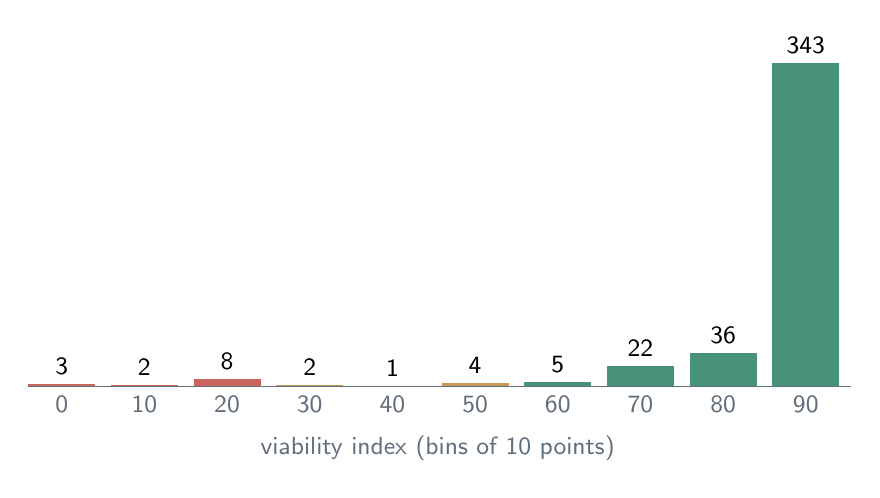
\begin{tikzpicture}[font=\sffamily\small,x=1cm,y=0.012cm]
  \foreach \i/\v in {0/3,1/2,2/8,3/2,4/1,5/4,6/5,7/22,8/36,9/343} {
    \pgfmathsetmacro{\x}{\i*1.05}
    \ifnum\i<3 \def\c{risk}\else\ifnum\i<6 \def\c{warn}\else\def\c{accent}\fi\fi
    \fill[\c!75] (\x,0) rectangle ++(0.85,\v);
    \node[above] at (\x+0.425,\v) {\v};
    \pgfmathtruncatemacro{\lo}{\i*10}
    \node[below,muted] at (\x+0.425,0) {\lo};
  }
  \draw[muted] (0,0) -- (10.45,0);
  \node[muted] at (5.2,-65) {viability index (bins of 10 points)};
\end{tikzpicture}
\caption{Viability index of 426 assessed companies. 179 score exactly 100. Bar colour indicates the index range; the level itself is set by the weakest dimension.}
\end{figure}

The distribution is intentionally skewed: most large US companies can pay their obligations, and the index does not invent differences among them. Its information sits in the tail.

\subsection{By sector}
\begin{center}\small
\begin{tabular}{@{}lrrrr@{}}
\toprule
Sector & viable & strained & at risk & not assessable \\
\midrule
Communication Services & 19 & 3 & 2 & -- \\
Consumer Discretionary & 42 & 1 & 4 & -- \\
Consumer Staples & 31 & 2 & 1 & -- \\
Energy & 21 & -- & -- & -- \\
Financials & -- & -- & -- & 76 \\
Health Care & 56 & 2 & 1 & -- \\
Industrials & 73 & 6 & 3 & 1 \\
Information Technology & 64 & 6 & 3 & -- \\
Materials & 24 & -- & 1 & -- \\
Real Estate & 25 & 5 & -- & -- \\
Utilities & 23 & 4 & 4 & -- \\
\bottomrule
\end{tabular}
\end{center}

\subsection{Companies at risk}
\begin{center}\small
\begin{tabularx}{\linewidth}{@{}lLr@{}}
\toprule
Weakest dimension & Companies (index) & n \\
\midrule
Shock absorption & Jabil (50.6), Carnival (39.4), Carvana (32.3), Atmos Energy (26.5), Builders FirstSource (25.5), Constellation Energy (25.1), Mosaic (24.4), PG\&E (24.4), Royal Caribbean (24.0), Huntington Ingalls (22.7), Norwegian Cruise Line (21.8), NRG Energy (19.3), EchoStar (5.9) & 13 \\
Cash generation & Sandisk (55.0), Boeing (50.3), Reddit (40.8), Moderna (7.4), Supermicro (5.8) & 5 \\
Debt service & Bunge (10.5) & 1 \\
\bottomrule
\end{tabularx}
\end{center}
Several of these reflect documented events rather than model artefacts: PG\&E's 2019--2020 wildfire bankruptcy, Atmos Energy's Winter Storm Uri costs in 2021, the cruise-line shutdown in 2020. Sandisk and Reddit have short histories that include cash-burning years.

\subsection{Strained}
Mostly two groups: companies with heavy but stable debt loads (Sempra, Simon Property Group, TransDigm, Deere, Dominion, Yum!\ Brands, Keurig Dr Pepper) and recent turnarounds whose ten-year record still contains cash-burn years (Netflix, Uber, Palantir, Vertiv, Western Digital).

\section{Does the index measure what it claims?}

The key test for the design goal is whether the index simply re-measures size or profitability. It should not.

\begin{center}
\begin{tabular}{@{}lrr@{}}
\toprule
Viability index vs. & Spearman $\rho$ & n \\
\midrule
Revenue (company size) & 0.03 & 424 \\
Net income (absolute profit) & 0.13 & 426 \\
Net margin (profitability) & 0.12 & 424 \\
Profit-weighted health score (attempt 1) & 0.49 & 426 \\
\bottomrule
\end{tabular}
\end{center}

Size and profit explain almost nothing of the ranking. The moderate correlation with the earlier health score is expected, because both contain cash flow and debt, but the two disagree exactly where profit and capacity diverge -- Intel, Delta and Carnival above. For comparison, the ``six months of cash'' draft still correlated $\rho = 0.32$ with margin.

\section{Limitations}
\begin{itemize}
  \item \textbf{Thresholds are judgement calls.} They are explicit and in one place, but not derived from outcome data.
  \item \textbf{No backtest yet.} The strongest non-speculative validation would compute the index as of fiscal 2019 and check whether it flagged the companies that needed emergency financing or cut staff in 2020.
  \item \textbf{Credit lines are not counted.} Undrawn revolving facilities are a real buffer but are tagged by only about 40 companies. The shock score is therefore conservative.
  \item \textbf{One repeat, one year.} The stress test covers a single repeat of the worst year, not a multi-year crisis.
  \item \textbf{History length.} Spin-offs and recent listings (Honeywell Aerospace, Paramount Skydance, Sandisk) have short or no histories.
  \item \textbf{Consolidated figures.} The index describes the group, not individual subsidiaries or regions where employees work.
  \item \textbf{Financial sector excluded} until regulatory capital data is added.
  \item \textbf{Utility data lags.} Several utilities' second-quarter 2026 filings were not yet in the XBRL API; their TTM ends in March 2026.
\end{itemize}

\section{How it could flow into the final ranking}

Because 42\,\% of assessed companies reach the maximum, the index is a poor differentiator among healthy companies -- by design. It is best used as a \textbf{gate or penalty}, not as another ranked indicator:
\[
\text{final score} = \text{sustainability score} \times f(\text{viability level}),\qquad
f = \begin{cases} 1.0 & \text{viable} \\ 0.7 & \text{strained} \\ 0.3 & \text{at risk} \\ 1.0 & \text{not assessable (flagged)} \end{cases}
\]
\begin{itemize}
  \item Above the threshold no company gains anything, so higher profit cannot improve a sustainability rank.
  \item A company that cannot keep paying its people cannot rank as sustainable, whatever its environmental record -- consistent with the ranking's multiplicative aggregation.
  \item \textbf{Keep the fixed thresholds.} Converting the index to within-sector ranks or z-scores before aggregation would reintroduce ``more is better'' and undo the design.
  \item In the Belastbarkeit (evidence-strength) view it would be its own evidence family: legally mandated SEC filings, weight 0.8.
  \item The factors 0.7 and 0.3 are placeholders to be decided by the team, ideally after the 2019$\rightarrow$2020 backtest.
\end{itemize}

\section{Reproduction}
\begin{verbatim}
python3 fetch_sec_facts.py <cache_dir>      # ~1 min, 1.8 GB, SEC fair-access rate
python3 financial_health.py <cache_dir>     # financial_health.csv (attempt 1)
python3 economic_viability.py <cache_dir>   # economic_viability.csv + bias check
\end{verbatim}
Python 3.9 standard library only. The SEC requires an identifying \code{User-Agent}; set \code{SEC\_USER\_AGENT}. Output columns include every intermediate value (years with positive cash flow, worst year and its size, shock cash flow, coverage, interest share, maturities), so each score can be traced back to the filings.

\end{document}
